\documentclass[a4paper,11pt]{article}
\usepackage[utf8]{inputenc}
\usepackage[T1]{fontenc}
\usepackage[normalem]{ulem}
\usepackage[english]{babel}
\usepackage{verbatim}
\usepackage{graphicx}
\usepackage{color} % définit une nouvelle couleur
\usepackage{float}
\usepackage[a4paper]{geometry}
\usepackage{hyperref}
\usepackage{bm, mathtools,amsmath, amssymb,upgreek}
\usepackage{tikz}
\geometry{hscale=0.8,vscale=0.8,centering}



\newcounter{manip}
\newenvironment{manip}[1][]{\refstepcounter{manip}\par\medskip
	\textbf{Manipulation~\themanip. #1} \rmfamily }{\medskip}

\newcounter{question}
\newenvironment{question}[1][]{\refstepcounter{question}\par\medskip
	\textbf{Question~\thequestion. #1} \rmfamily }{\medskip}


\definecolor{QuestionColor}{rgb}{0.9,0.95,1} % bleu ciel
\definecolor{SolutionColor}{rgb}{0.9,0.95,1} % bleu ciel


\newcommand{\be}{\begin{equation}}
\newcommand{\ee}{\end{equation}}
\newcommand{\bea}{\begin{eqnarray}}
\newcommand{\eea}{\end{eqnarray}}
\newcommand{\MI}{|\rm{MI}\rangle}
\newcommand{\SF}{|\rm{SF}\rangle}
\newcommand{\ah}{\hat{a}}
\newcommand{\ac}{\hat{a}^\dag}


\title{Lab Work \\ CPT-based Cs microcell atomic clock}
\author{}
\date{2019}
\begin{document}
\maketitle

\tableofcontents 

\section{Basics on miniature atomic clocks}
Figure \ref{fig:globalcpt} shows the architecture of a miniature Cs cell atomic clock based on coherent population trapping (CPT).

\begin{figure}[h!]
	\centering
	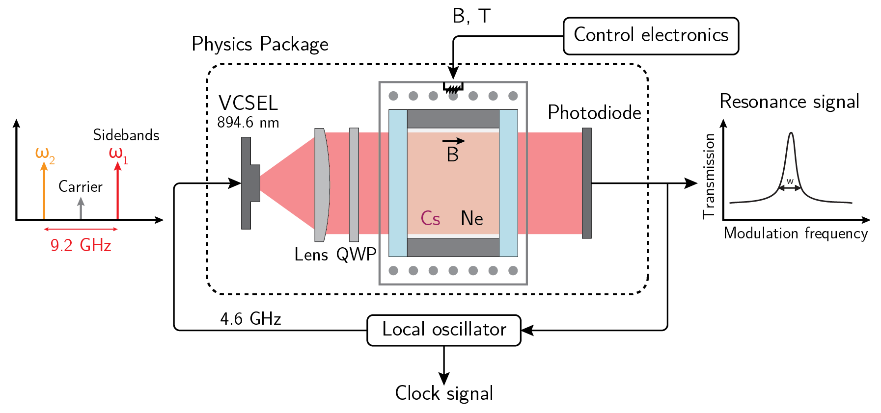
\includegraphics[width=0.7\linewidth]{globalCPT}
	\caption{Simplified architecture of a buffer-gas filled Cs microcell CPT atomic clock.}
	\label{fig:globalcpt}
\end{figure}

Cs vapor is filled in a glass-silicon-glass micro-fabricated cell whose technology is described in~\cite{hasegawa}. The Cs cell is filled with a pressure buffer gas. The buffer gas slows down atoms in the microcell and increases the time for the atoms to reach the cell walls. It also reduces the first-order Doppler effect and leads to operation in the Lamb-Dicke regime~\cite{dicke}. Eventually, it helps to detect narrow CPT resonances.

Atoms in the cell interact with a dual-frequency (in the ideal case!) optical field generated by a VCSEL laser whose injection current is directly modulated at 4.596 GHz through a bias-tee. This generates two first-order optical sidebands separated by about 9.192 GHz, required to produce the CPT interaction. The laser output beam crosses a neutral density filter to attenuate the optical power and a quarter-wave plate to polarize circularly the optical beam. The light transmitted through the cell is detected by a photodiode.

When the frequency difference between both first-order optical sidebands exactly equals the Cs ground-state hyperfine splitting (9.192 631 770 GHz), atoms are trapped through a quantum interference process in a quantum superposition of both ground states (see Fig.~\ref{fig:ppeCPT}). In this so-called dark state, the light atomic absorption is reduced and the atomic vapor transparency is increased. The CPT resonance linewidth is ultimately limited by the microwave CPT coherence relaxation time and can be measured to be of about 1 kHz in a buffer-gas filled micro-fabricated cell. The signal at the output of the photodiode is used in two main servo loops. The first one is dedicated to the stabilization of the laser frequency onto the bottom of a homogeneously broadened optical line. The second loop stabilizes the local oscillator (LO) frequency onto the atomic clock transition.

\begin{figure}[h!]
	\centering
	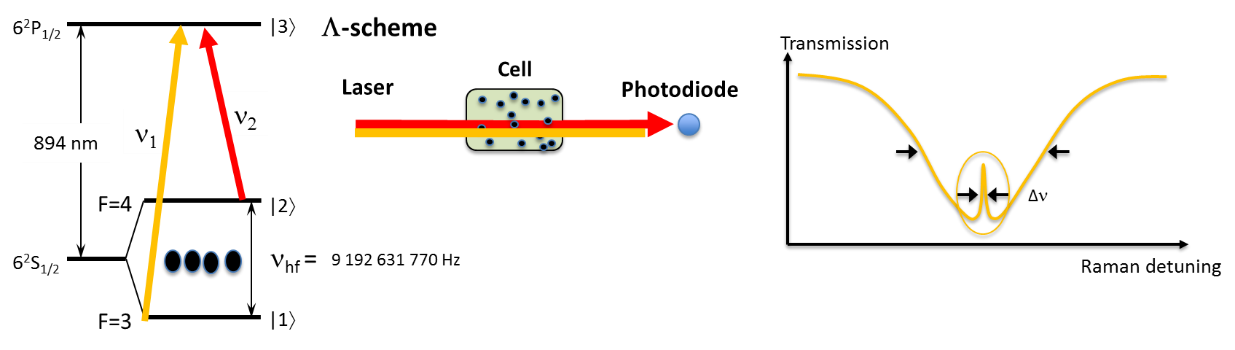
\includegraphics[width=0.9\linewidth]{ppeCPT}
	\caption{Basic principle of CPT.}
	\label{fig:ppeCPT}
\end{figure}


\section{Presentation of the CPT clock experiment}
Figure~\ref{fig:environnement} shows the table-top experiment environment.

\begin{figure}[h!]
	\centering
	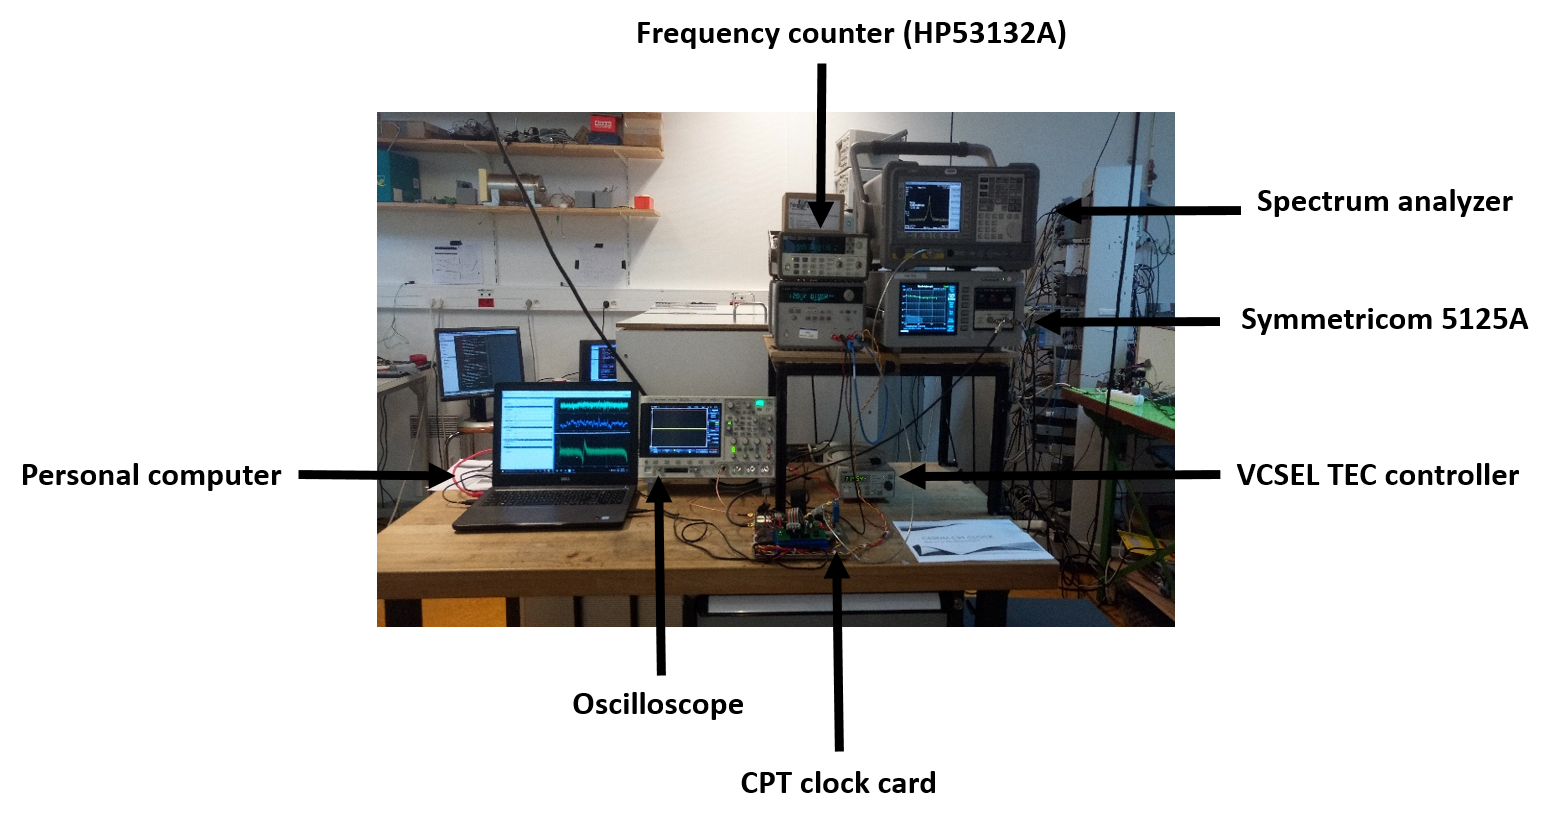
\includegraphics[width=0.9\linewidth]{environnement}
	\caption{Table-top CPT experiment environment. From left to right: personal computer to pilot the experiment, 		oscilloscope to monitor signals, the CPT clock card including physics package and all embedded electronics, a Thorlabs 		TEC200C controller used to stabilize the VCSEL temperature. On the top-right, a power-supply to drive the clock-card, 		a frequency counter (HP53132A), a spectrum analyzer used to monitor the local oscillator microwave signal at 4.6 GHz 		and a Symmetricom 5125A test-set to measure the clock Allan deviation. A hydrogen maser 10 MHz signal cable is also 		available.}
	\label{fig:environnement}
\end{figure}

Figure~\ref{fig:clock-card} shows a zoom on the clock-card.

\begin{figure}[h!]
	\centering
	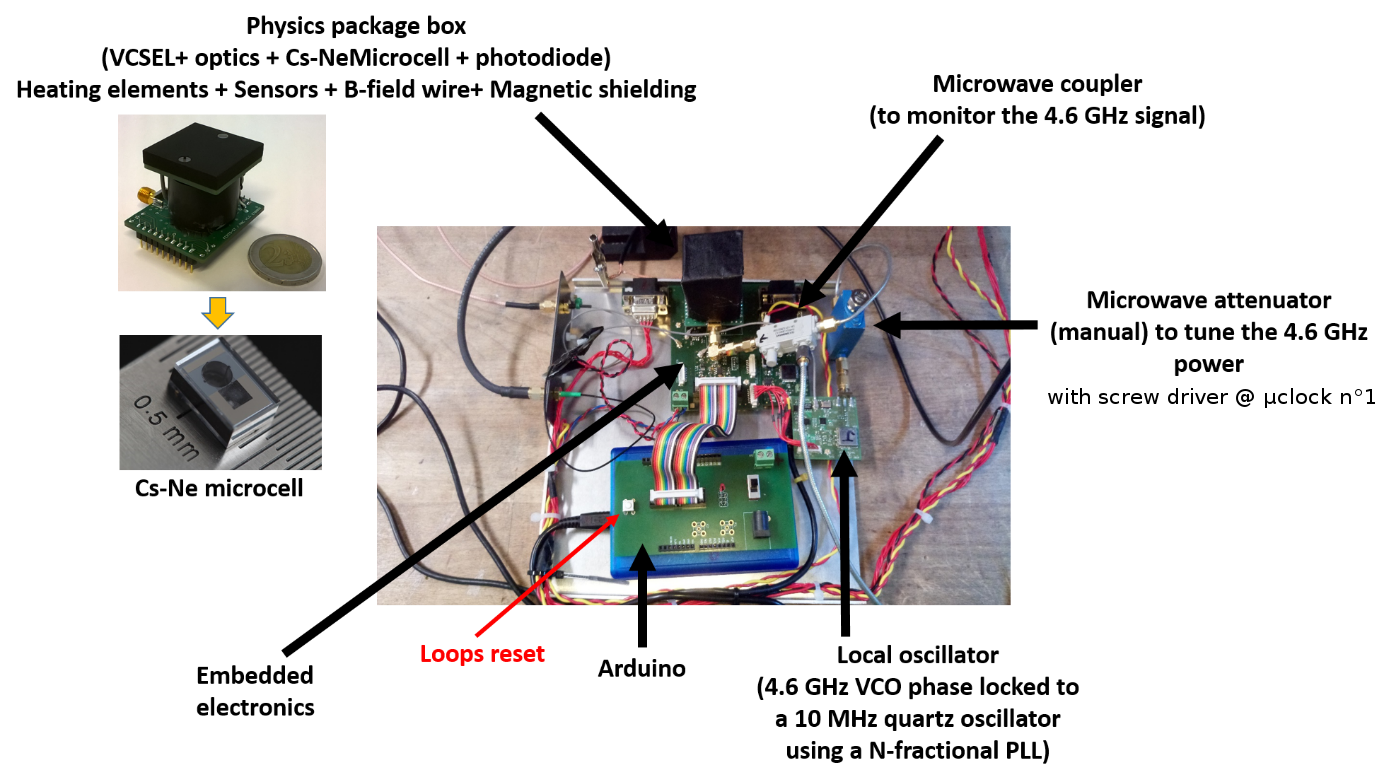
\includegraphics[width=0.9\linewidth]{clock-card}
	\caption{Details of the clock-card.}
	\label{fig:clock-card}
\end{figure}


{\bf Important points: }

VCSEL : 894.6 nm (Cs D1 line) 
Microcell: Cs-Ne ($\approx 76$~Torr), heated at about 75$^\circ$C. The cell length is 1.4~mm. Its diameter is 2~mm.
The static magnetic field applied along the cell can be tuned using a current value. It is applied in order to lift the Zeeman degeneracy. 

Figure~\ref{fig:gui} shows the typical interface program window to pilot the clock. A C program was implemented to pilot a microcontroller through an Arduino platform. A preliminary Python interface was developed to operate the clock. You can visualize the commands and digital words sent to the micro-controller at any time in the command window.

\begin{figure}[h!]
	\centering
	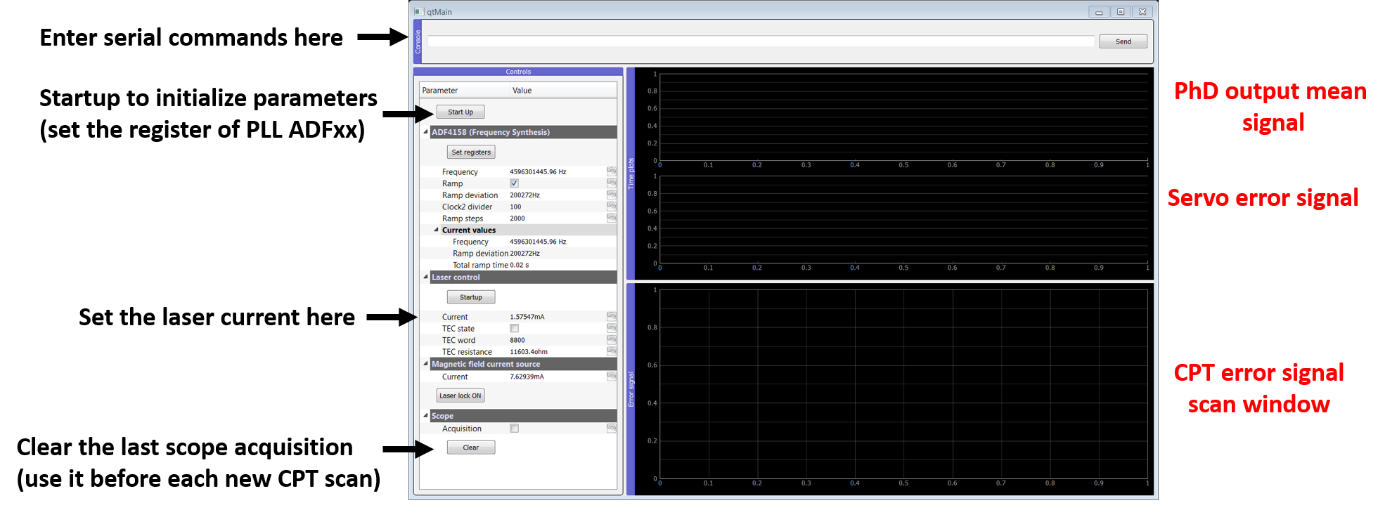
\includegraphics[width=0.9\linewidth]{gui}
	\caption{Program graphic interface.}
	\label{fig:gui}
\end{figure}

The program is launched from a Jupyter Notebook which should be already running on your labwork computer.


\section{Lab work}
\subsection{Open the main program interface}
The graphical interface is ran from a jupyter notebook which will be already running when you start the labwork. 

In case you need to restart the interface, simply chose the “Restart and Clear Output” under the “Kernel” menu, and re-run the first cell of the notebook.

With the Jupyter Notebook, you can execute code and/or plot your data in the same session.

\subsection{Initial configuration}
The laser temperature set-point has been pre-set using the Thorlabs TED200C. It is set at 22$^\circ$C (11.364 k$\Omega$) for the J clock, around 70$^\circ$C (1.816 k$\Omega$) for the TP1 clock and around 80$^\circ$C (1.259 k$\Omega$) for the TP2 clock.
For the first step, the 4.6 GHz signal power is turned off by the microwave attenuator at the output of the local oscillator card (the sliders 1 to 6 are set to “1”, see Fig.~\ref{fig:attenuation} and Fig.~\ref{fig:attenuation-table}).



\begin{figure}[h!]
	\centering
	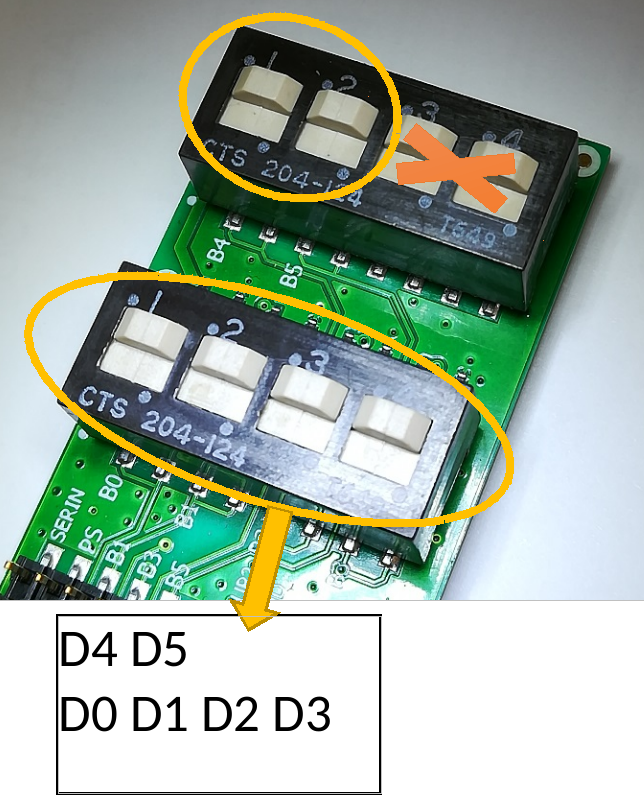
\includegraphics[width=0.5\linewidth]{attenuation}
	\caption{Localization of the sliders for the 0.1 GHz to 6.0 GHz, 0.5 dB LSB, 6-bit, silicon digital attenuator. MSB = Most Significant Bit, LSB = Least Significant Bit.}
	\label{fig:attenuation}
\end{figure}

\begin{figure}[h!]
	\centering
	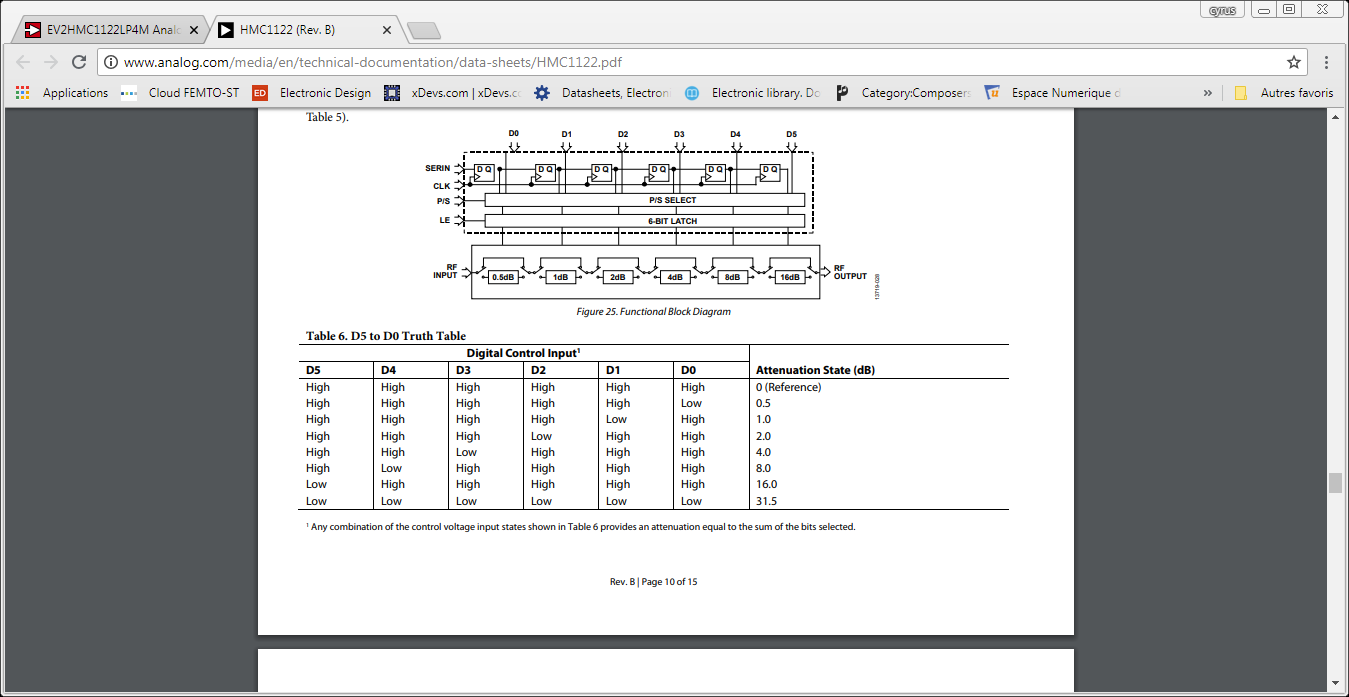
\includegraphics[width=0.9\linewidth,trim={7cm 4.2cm 12cm 9.1cm},clip]{attenuation-table}
	\caption{Attenuation table for the 0.1 GHz to 6.0 GHz, 0.5 dB LSB, 6-bit, silicon digital attenuator.}
	\label{fig:attenuation-table}
\end{figure}

\subsection{VCSEL diode laser response}

\begin{manip}
Change the laser current from 0 to 1.7 mA by 0.1 mA steps and measure the photodiode output voltage with the oscilloscope. Do not exceed I=1.8 mA (for VCSEL protection) for the VCSEL dc current. To set the current, you can directly enter a value in mA in the “current” box.
Store your values in your labwork dedicated .txt file, which you can open using the command window and typing:
\begin{verbatim}
G:\users\cyrus.rocjer\NextCloud\MAC control program\labwork>lvi-x.txt
\end{verbatim}
Where x=1, 2 or J depending on your setup.
You can then use the Jupyter notebook for plotting, by restarting and clearing the kernel and then running the 2nd and 3rd cells of the notebook consecutively.
Identify the current value right above threshold. Set the diode current at this value and write down the digital word xxxxx sent to the Arduino in the Command Window.
\end{manip}

\subsection{Linear spectroscopy}

\begin{manip}
	Tune the laser current above the lasing threshold using the laser control box interface. 
	The goal is now to sweep the laser frequency. For this purpose, we apply a ramp voltage onto the laser current to sweep the laser frequency. For information, the ramp is composed of 5000 pts. To do this, enter in the serial command window:
	\begin{verbatim}
	t xxxxx s
	\end{verbatim}
	
	\texttt{t} calls the ramp function;
	
	\texttt{xxxxx} is the laser current (digital word) starting point, which you have measured above;
	
	\texttt{s}  calls a scan function.
	
	Look at the spectrum obtained on the oscilloscope. If required, tune the starting point by changing the digital word. Explain what you observe. 
\end{manip}

\begin{question}
	Identify and name the different optical transitions of the Cs $D_1$ line. For reminder, the figure~\ref{fig:Cslevels} reports the Cs $D_1$ line energy structure. Identify the transitions 3-3’, 3-4’, 4-3’ and 4-4’.
\end{question}

\begin{figure}[h!]
	\centering
	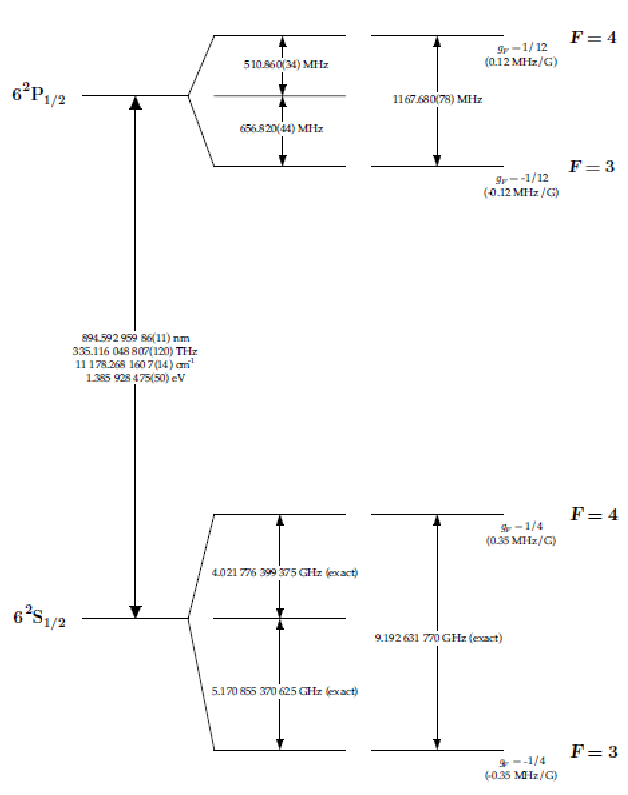
\includegraphics[width=0.9\linewidth]{Cslevels}
	\caption{Atomic levels of Cs.}
	\label{fig:Cslevels}
\end{figure}


\begin{question}
	 Calibrate the x-axis to determine roughly the laser frequency variation for a basic digital step.
\end{question}

\begin{question}
Measure the linewidths of the optical transitions. Given the cell temperature $T\approx80^{\circ}C$ and the Neon buffer gas broadening coefficient $\beta \approx 11 \ \rm{MHz/Torr}$, estimate the buffer gas pressure $p$.
\end{question}

\begin{question}
Estimate the optical absorption of the cell (the percentage of laser power absorbed by the cell). The Beer-Lambert law, assuming that we operate in an optically thin medium, could help you to estimate the actual cell temperature. Here, knowing the cell length $L=1.4 \ \rm{mm}$ and the broadened linewidth, you can estimate the Cs atomic density inside the cell and the Cs partial pressure $p_{Cs}$.
\end{question}

\textbf{Note:} one could fit this spectrum by a sum of four Voigt profiles to estimate the absorption lines broadening. This broadening results from the sum of the optical transition natural linewidth, the Doppler broadening and an additional broadening due to the presence of buffer gas. By using the optical density and the line broadening measurements, one can extract both the temperature and buffer gas pressure of a particular cell.
Here, you can estimate the expected Doppler broadening and see how different your measured linewidth is.

\begin{equation}
\Delta \nu_D = \frac{2\nu_{\rm opt}}{c}\sqrt{\frac{2 R T}{M}\ln 2},
\end{equation}
with $\nu_{\rm opt}=335$~THz, $R=8.31$~J/(mol.K), $M=133$~g/mol.

\subsection{Towards CPT spectroscopy}
We now start to implement CPT spectroscopy. 

\begin{manip}
Now turn on the 4.6 GHz microwave signal and increase progressively its power using the microwave attenuator. To do this, you can set the attenuators sliders to 0, starting from the bottom-left slider. Note that you can read the actual microwave power by monitoring the spectrum analyzer. This measured power is 20 dB (20dB-coupler) lower than the one actually experienced by the VCSEL bias tee. 
\end{manip}

\begin{question}
	What do you observe? Explain.
\end{question}

Set the microwave power (read on the spectrum analyzer) to - 25 dBm.
To detect a CPT signal, we need to ensure that the laser frequency is tuned (ideally “stabilized” in a real miniature atomic clock using a lockin amplifier-based modulation-demodulation technique applied on the laser current) such that the laser is connected to a given excited state. 
For this purpose, the laser frequency must be adjusted such that the photodiode output signal is tuned on the bottom of a “CPT-resonant” broadened optical line (the one that appeared between both initial doublets of the Cs D1 line!). 

\begin{question}
You first need to determine roughly the diode current value at the bottom of the central absorption line. To do so, use your knowledge of the scanning ramp.
\end{question}

\begin{manip}
Switch off the laser ramp (use the reset button on the clock card, shown by the red arrow in figure~\ref{fig:clock-card}).

Apply the serial command:

\texttt{9 xxxxx}

\texttt{9} calls a function to fix the laser dc current
\texttt{xxxxx} is the digital word, image of the laser dc current 

Check that the photodiode output voltage is well-driven to the bottom of the absorption line. If not, change the digital word by a few 10s.

Once the laser frequency is well-adjusted, you can first lock the laser using a simple linear absorption lock. To do so, type ‘\texttt{3}’ in the command line. 
\end{manip}

\begin{question}
Comment on what happens on the photodiode signal. Write down the digital word where the laser lock has stabilized.
\end{question}

\begin{manip}
Once the laser frequency is well-adjusted, we can try to detect the CPT resonance by scanning the local oscillator frequency. For this purpose, Press the “Reset” button on the clock card and click the “Clear” button and enter the serial command:  

\texttt{b}  

As you can see on the spectrum analyzer, this command allows to sweep the local oscillator frequency by about 100 kHz.  This value is the typical span of the “CPT error signal scan window” in the bottom of the program interface. The central frequency was fixed here to about 4.596340xxx GHz. 
Here, you should detect the CPT signal (CPT error “demodulated” signal in fact) in the bottom CPT error signal scan window. Note that the signal to noise ratio of the CPT signal can be significantly increased by tuning finely the laser optical detuning (command \texttt{9 xxxxx} where \texttt{x} is the laser current digital word).  
\end{manip}


\begin{question}
	Estimate the CPT signal linewidth in Hz and the CPT signal amplitude (arb. units).
	\end{question}


\begin{manip}
Do this measurement for several values of the 4.6 GHz signal power (-29 to -24 dBm) and note for each case the CPT signal amplitude. 
Note: Each time you change the microwave power, re-adjust the laser current to be on the bottom of the good optical absorption line (serial command: \texttt{9 xxxxx}), click the Clear button and turn on the LO ramp (serial command \texttt{b}).
\end{manip}


\begin{question}
Plot the CPT signal amplitude (arb. units) versus the microwave power. Explain the result.
\end{question}


\begin{manip}
Reduce now the value of the static magnetic field current. What do you observe? Record the CPT spectrum for a few values of the static magnetic field. This measurement could help you to know the actual static magnetic field experienced by the atoms. Indeed, magnetic-sensitive Zeeman transitions are shifted by about 700 kHz/G. 

From this, note that the best way to know the actual magnetic field variations experienced by the atoms is to stabilize the LO frequency onto one the magnetic-field sensitive Zeeman transition. In this case, fluctuations of the clock frequency are expected to be mainly due to this effect.\\
\end{manip}


\subsection{Close the atomic clock loop}

\begin{manip}
Set the microwave power at -25 dBm.
Tune the laser current to the bottom of the good absorption line (serial command: \texttt{9 xxxxx}).

Enter the serial command \texttt{i xxxxx}.

Enter the serial command \texttt{0}.
\end{manip}

The latter command allows to stabilize both the laser frequency and the local oscillator frequency onto the CPT resonance frequency. For both servo loops, a digital lock-in amplifier technique is applied. In clock closed loop operation, the frequency synthesizer is used to scan successively on both sides of the CPT resonance. An error signal, proportional to the Raman detuning, is generated and processed in a PI controller system to correct the 10~MHz quartz oscillator pilot frequency (quartz voltage tuning). The output useful signal is the signal from the 10 MHz quartz oscillator, locked to the atoms.


\begin{manip}
Check that the servo loop is OK (stabilization of the laser current and LO frequency going to the correct frequency).
\end{manip}


\begin{manip}
	You can then measure the clock Allan deviation using the Symmetricom test setup (see Fig.~\ref{fig:allan}).
\end{manip}

\begin{figure}[h!]
	\centering
	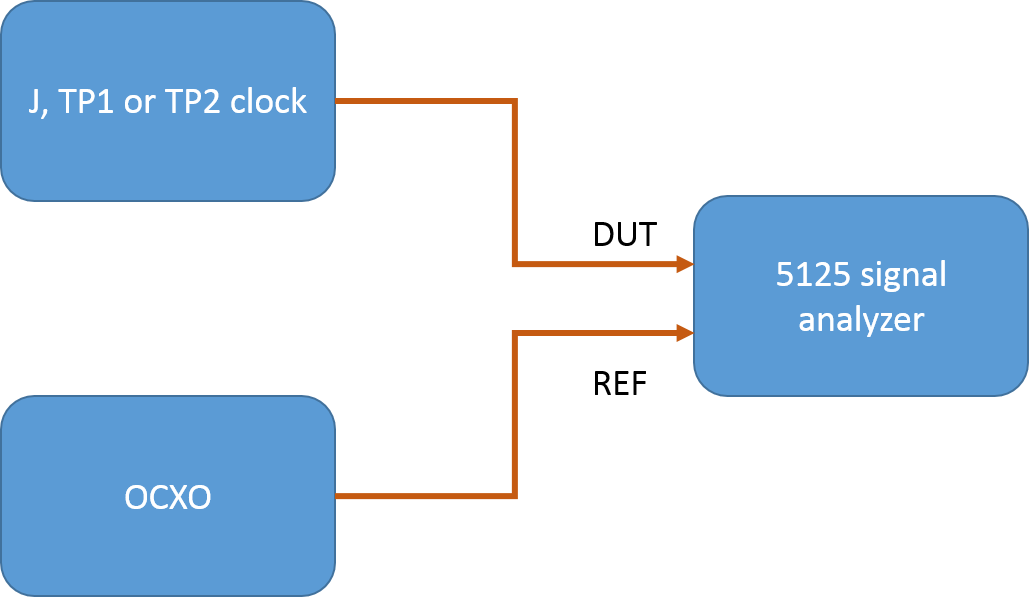
\includegraphics[width=0.9\linewidth]{allan}
	\caption{Clock Allan deviation measurement setup.}
	\label{fig:allan}
\end{figure}


\begin{manip}
	To do so, we will compare the labwork clocks with very stable OCXOs (oven-controlled quartz oscillators). Before measuring the clock fractional frequency instability, it is necessary to verify the OCXO performance. To do so, one can input two different OCXO signals to the 5125 signal analyzer.
	
	You can then plug the clock LO signal at 10 MHz to the DUT port, while the OCXO signal at 5 MHz is sent to the REF port. Establish the clock short-term performance, as well as the OCXO frequency drift.
	
	You can then compare short-term stability performances in both free-running and locked regimes.
\end{manip}

\begin{question}
	How would you estimate the clocks stability if you did not have a good OCXO to compare it to? Propose a first measurement that can help obtaining an estimate using two clocks.
	
	Is there a way to know the actual individual clocks stabilities given that there are four Labwork clocks?
\end{question}

\begin{manip}
	If there is any time left, you can go ahead and try to use one of the two above solutions.
\end{manip}

\section{Appendices}
\subsection{VCSEL laser response}
\begin{figure}[h!]
	\centering
	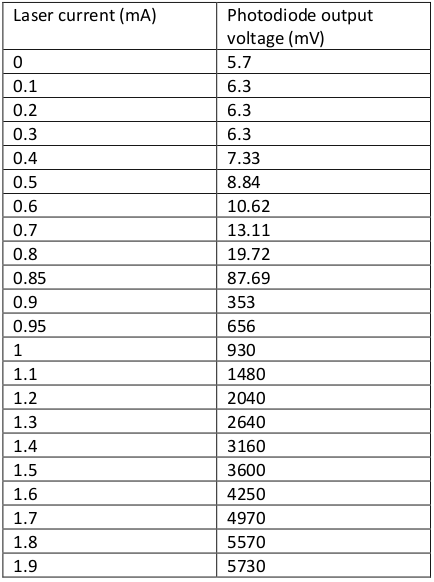
\includegraphics[width=0.6\linewidth]{vcsel-response}
	\caption{}
	\label{fig:vcsel-response}
\end{figure}

The laser threshold current is measured to be about 0.8 mA (see Fig.~\ref{fig:threshold}).
\begin{figure}[h!]
	\centering
	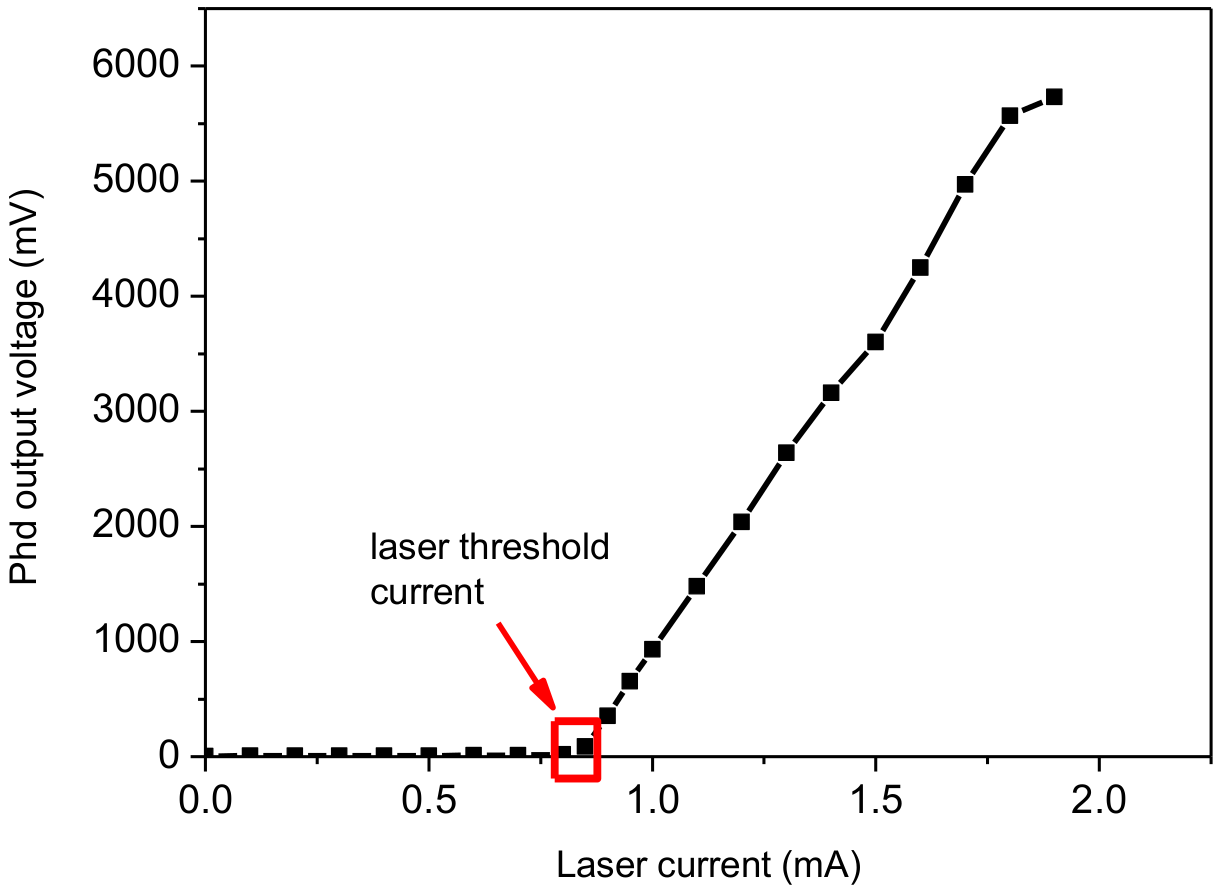
\includegraphics[width=0.5\linewidth]{threshold}
	\caption{}
	\label{fig:threshold}
\end{figure}

\subsection{Absorption spectrum of the Cs D 1 line (without 4.6 GHz)}
See Fig.~\ref{fig:absorption1}
\begin{figure}[h!]
	\centering
	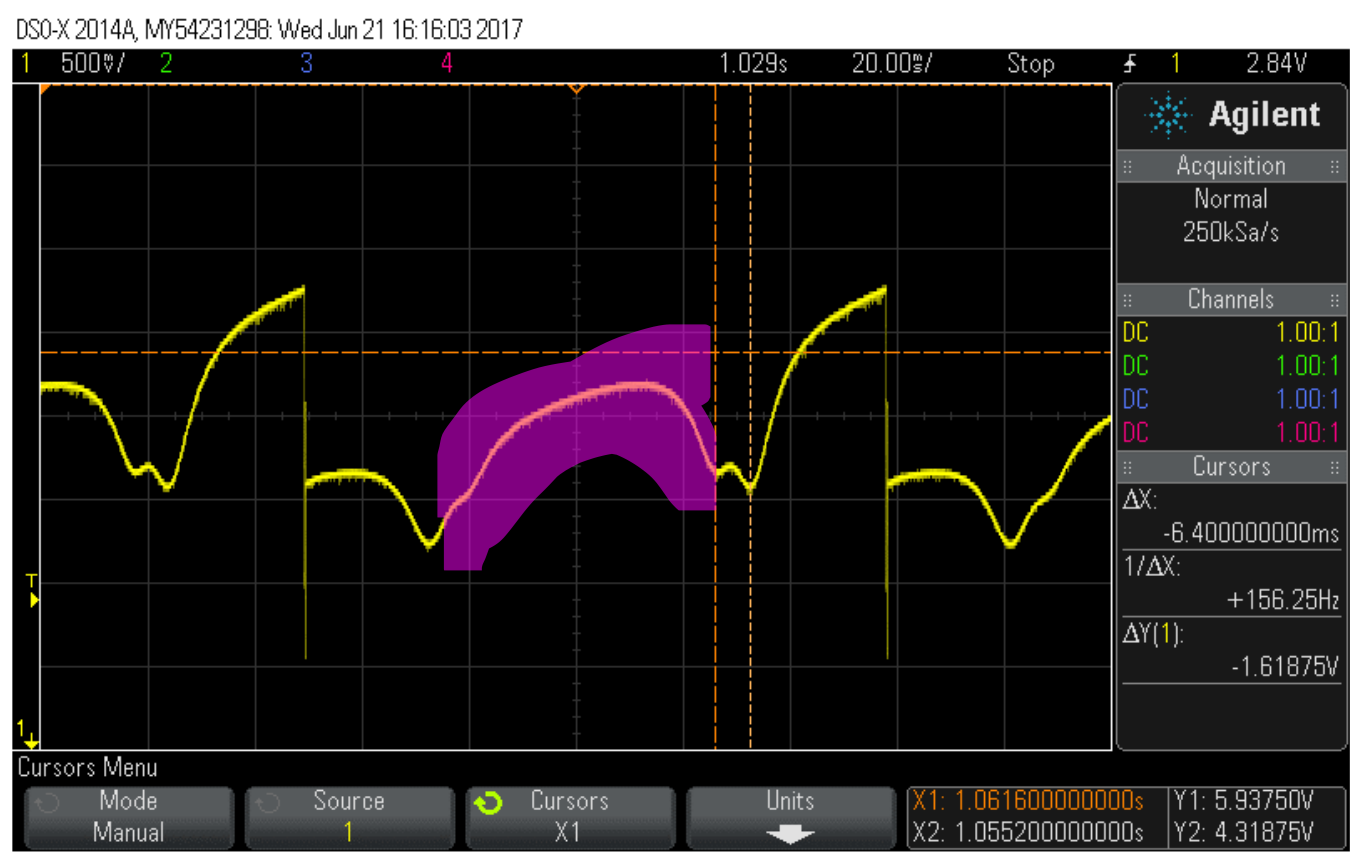
\includegraphics[width=0.5\linewidth]{absorption1}
	\caption{Without RF}
	\label{fig:absorption1}
\end{figure}
We find: 5000pts of the ramp = 108.8 ms.
Moreover, 1.167 GHz = 6.4 ms et 9.192631770 GHz = 54 ms.
We deduce: 5000 pts = 18.521 450 677 GHz, yielding 1 pt = 3.704 MHz of laser frequency.

Nothing interesting on the purple area....


\subsection{Towards CPT spectroscopy}
See Figs.~\ref{fig:absorption2} and \ref{fig:errorsignal}
\begin{figure}[h!]
	\centering
	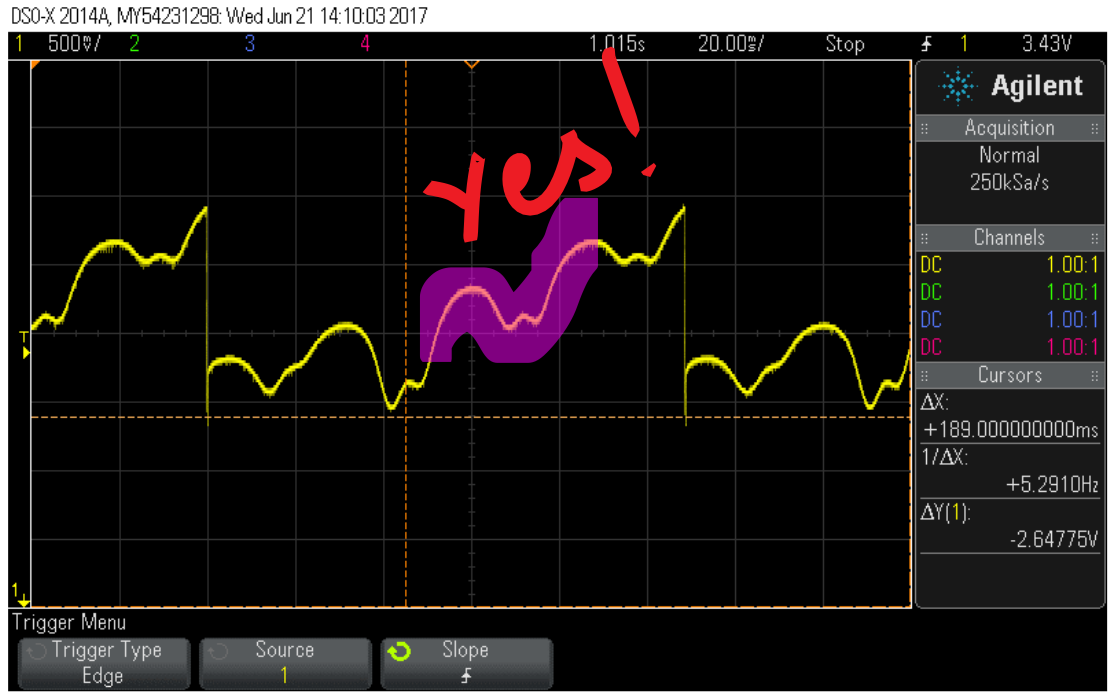
\includegraphics[width=0.5\linewidth]{absorption2}
	\caption{With RF}
	\label{fig:absorption2}
\end{figure}
We see CPT lines!
The application of the 4.6 GHz microwave signal makes appear a doublet between both initial doublets. CPT
spectroscopy

\begin{figure}[h!]
	\centering
	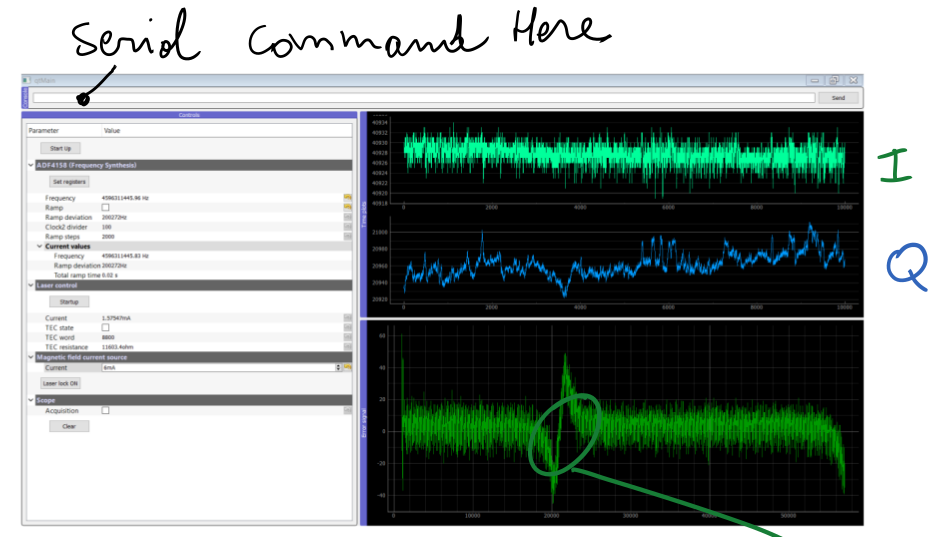
\includegraphics[width=0.5\linewidth]{errorsignal}
	\caption{CPT error signal}
	\label{fig:errorsignal}
\end{figure}


\subsection{Close the loops}

Serial Commands reminder (see Fig.~\ref{fig:reminder}):
\begin{figure}[h!]
	\centering
	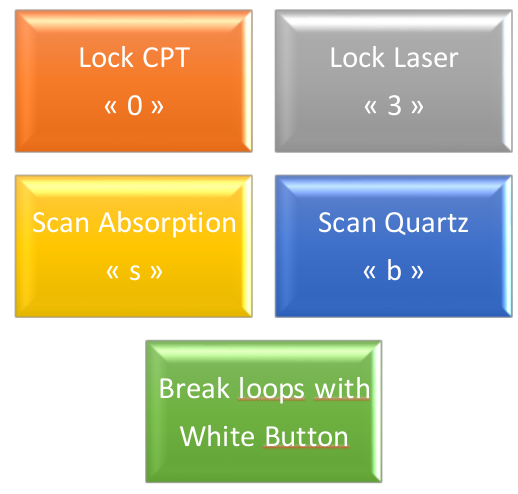
\includegraphics[width=0.5\linewidth]{reminder}
	\caption{}
	\label{fig:reminder}
\end{figure}





\begin{thebibliography}{9}
	
	\bibitem{hasegawa}
	M. Hasegawa et al., Sensors Actuators 167, 594-601 (2011)
	
	\bibitem{dicke}
	R. H. Dicke, Phys. Rev. 89, 472 (1953)
	
\end{thebibliography}


\end{document}
